\documentclass[15,a4paperpaper,]{article}

  \title{MRC/WITS-AGINCOURT UNIT STUDY AREA HDSS FACT SHEET}
  \author{Agincourt}
  \date{}
  


\newcommand{\logo}{logo.png}
\newcommand{\cover}{cover.png}
\newcommand{\iblue}{2b4894}
\newcommand{\igray}{d4dbde}

% Author: Karol KozioL
% License: GPL-3
% Modified by: Sarah Wagner

% % % packages -----------------------------------------------------------------------------------
\usepackage{amsmath}
\usepackage{array}
\usepackage{booktabs}
\usepackage{calc}
\usepackage{eso-pic}
\usepackage{fancyhdr}
\usepackage{fontspec}
\usepackage[left = 2.5cm, right = 2.5cm, top = 1.2cm, bottom = 1.2cm, includeheadfoot]{geometry}
\usepackage{graphicx}
\usepackage[utf8]{inputenc}
\usepackage{lastpage}
\usepackage{multirow}
\usepackage{tabularx} 
\usepackage{tikz}
\usepackage{titlesec}
\usepackage{xcolor, colortbl}

% % % settings -----------------------------------------------------------------------------------

% % custom colors
\definecolor{iblue}{HTML}{\iblue}
\definecolor{igray}{HTML}{\igray}

% definition of pagename
\newcommand\pagename{Page}

% % fonts 
\defaultfontfeatures{Mapping = tex-text}
\setmainfont[BoldFont = Lato-Bold.ttf, ItalicFont = Lato-Italic.ttf, BoldItalicFont = Lato-BoldItalic.ttf]{Lato-Regular.ttf}
\newfontfamily\headingfont[ItalicFont = Lato-BlackItalic.ttf]{Lato-Black.ttf}


% % sections
\titleformat{\section}{\color{iblue}\headingfont\Large\bfseries}{\thesection}{1em}{}[\titlerule]
\titleformat{\subsection}{\color{iblue}\headingfont\large\bfseries}{\thesubsection}{1em}{}
\titleformat{\subsubsection}{\color{iblue}\headingfont\bfseries}{\thesubsubsection}{1em}{}

% % misc
\setlength{\parindent}{0em} 
\linespread{1}
\raggedright
\newcolumntype{C}{>{\centering\arraybackslash}X}


% % % custom titlepage ----------------------------------------------------------------------------
\newcommand\BackgroundPic{%
	\put(0,0){%
		\parbox[b][\paperheight]{\paperwidth}{%
			\vfill
			\centering
			
\includegraphics[width=\paperwidth,height=\paperheight]{\cover}%
			\vfill
}}}

\makeatletter

% pagestyle titlepage
\fancypagestyle{customtitle}{
	\lhead{}
	\chead{}
	\rhead{}
	\makeatother
	\lfoot{}
	\cfoot{}
	\rfoot{
\includegraphics{\logo}}
}


% titlepage
\renewcommand{\maketitle}{
	\thispagestyle{customtitle}
	\AddToShipoutPicture*{\BackgroundPic}
	\ClearShipoutPicture
	
	\phantom{a}\hfill
	\vspace{14cm}
	
	\begin{tabular}[l]{@{}p{\textwidth}@{}}
		\color{iblue}\headingfont\LARGE\@title\\[1em]
		\color{iblue}\headingfont\large\@author\\[1em]
		\color{iblue}\headingfont\small\@date\\[1em]
	\end{tabular}
	
	
	
	\clearpage
}
\makeatother

% % % header and footer ---------------------------------------------------------------------------
\pagestyle{fancy}
\lhead{}
\chead{}
\rhead{ 
\includegraphics{\logo}}
\makeatother
\newlength{\myheight}
\lfoot{}
\cfoot{}
\rfoot{\pagename~\thepage \hspace{1pt} / \pageref{LastPage}}
\renewcommand\headrulewidth{0pt}
\renewcommand\footrulewidth{0pt}




\begin{document}


\renewcommand{\contentsname}{Sections}

\renewcommand{\pagename}{Seite}


\maketitle

\addcontentsline{toc}{section}{Contents}
\clearpage

\section{Introduction}

This ``Fact Sheet'' provides basic information on the population and
demographics for the Agincourt HDSS study area using data from the 2019
and 2020 annual updates across all villages in the study area. Whenever
you use this information, please reference it as being obtained from
MRC/Wits Rural Public Health and Health Transitions Research Unit
(Agincourt).

\emph{Villages in the Agincourt Health and Socio-Demographic
Surveillance (HDSS) System study area in 2019/2020 include}:\\
Agincourt, Belfast, Croquet Lawn, Croquet Lawn B, Cunningmore A,
Cunningmore B, Dumphries A, Dumphries B, Dumphries C, Huntington, Ireagh
A, Ireagh B, Ireagh C, Justicia, Khaya Lami, Kildare A, Kildare B,
Kumani, Lillydale A, Lillydale B, Makaringe, MP Stream, Newington B,
Newington C, Rolle C, Somerset, Somerset C, and Xanthia.

Where is Agincourt village in the MRC/Wits-Agincourt Unit Health and
socio-Demographic System (HDSS) study area?

\includegraphics{/Users/Chido/Pictures/Agincourt HDSS.jpg}

\section{Agincourt village population 2020}

The numbers shown below are calculated according to numbers for the end
of June 2020. The numbers are known as mid-year population figures.

\begin{table}[ht]
\centering
\begin{tabularx}{\textwidth}{|l|C|}
  \rowcolor{igray} \hline
Category & Total \\ 
  \hline
Households & 1309 \\ 
  Population & 6917 \\ 
  Male & 3395 \\ 
  Female & 3522 \\ 
  Children under 5 & 592 \\ 
  Children of school-going age (5-19) & 1153 \\ 
   \hline
\end{tabularx}
\end{table}

\pagebreak

Below you can see how many people were living in Agincourt of different
ages in June 2020.

\begin{table}[ht]
\centering
\begin{tabularx}{\textwidth}{|l|C|C|C|}
  \rowcolor{igray} \hline
Age group & Male & Female & Total \\ 
  \hline
0-4 & 305 & 287 & 592 \\ 
  5-9 & 332 & 334 & 666 \\ 
  10-14 & 353 & 362 & 715 \\ 
  15-19 & 312 & 311 & 623 \\ 
  20-24 & 303 & 327 & 630 \\ 
  25-29 & 364 & 333 & 697 \\ 
  30-34 & 350 & 312 & 662 \\ 
  35-39 & 278 & 247 & 525 \\ 
  40-44 & 204 & 201 & 405 \\ 
  45-49 & 148 & 157 & 305 \\ 
  50-54 & 107 & 133 & 240 \\ 
  55-59 & 107 & 145 & 252 \\ 
  60-64 &  74 & 108 & 182 \\ 
  65-69 &  59 &  80 & 139 \\ 
  70-74 &  36 &  59 &  95 \\ 
  75-79 &  26 &  40 &  66 \\ 
  80-84 &  25 &  31 &  56 \\ 
  85-89 &   6 &  19 &  25 \\ 
  90-94 &   3 &  26 &  29 \\ 
  95+ &   2 &  10 &  12 \\ 
   \hline
\end{tabularx}
\end{table}

Additionally, you can also see the population structure of Agincourt for
2020.

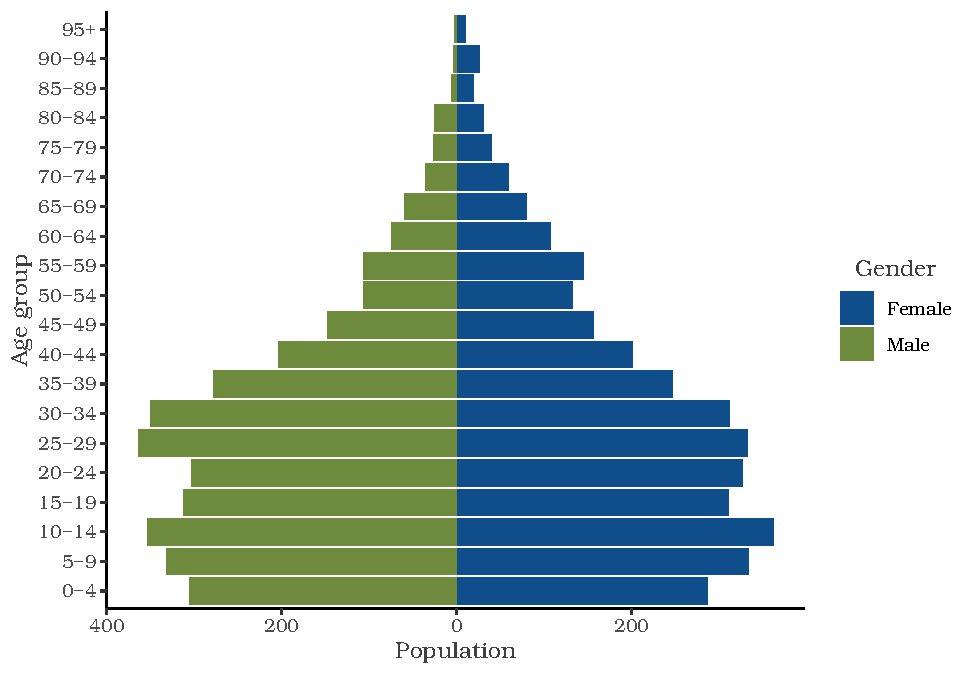
\includegraphics{mainfactsheet_files/figure-latex/unnamed-chunk-6-1.pdf}

\pagebreak
\section{Births}

\subsection{Number of Births by Sex}

The number of births recorded in Agincourt are shown below. We can only
provide data to the end of 2019.

\begin{table}[ht]
\centering
\begin{tabularx}{\textwidth}{|l|C|}
  \rowcolor{igray} \hline
Category & Count \\ 
  \hline
Male Births &  39 \\ 
  Female Births &  47 \\ 
  Total Births &  86 \\ 
   \hline
\end{tabularx}
\end{table}

\subsection{Crude Birth Rate (how many babies born for every one thousand people)}

The text makeover below shows the crude birth rates in Agincourt in
2019.

~\\
\begingroup \fontfamily{ppl}\fontsize{70}{70}\selectfont
\textbf{\textcolor{olive}{12}} \endgroup \begingroup
\fontsize{30}{30}\selectfont \textcolor{olive}{live births} were

observed on average out

\textcolor{olive}{of every 1000 of the population}

in Agincourt in the year 2019 \endgroup

~\\
\hspace*{0.333em}\\
The crude birth rate is found by comparing the number of babies born to
the total population. For every 1 000 people (all ages and both male and
female) living in Agincourt in the year of 2019, 12 babies were born.

\subsection{Births by Mother's Age and Age Specific Fertility Rates (ASFR)}

Research within the MRC/Wits-Agincourt Unit HDSS study area continues to
look closely at fertility. You can see the number of babies born to
mothers of different ages in the study area in 2019 below.

\begin{table}[ht]
\centering
\begin{tabularx}{\textwidth}{|l|C|}
  \rowcolor{igray} \hline
AgeGroup & ASFR \\ 
  \hline
10-14 & 8.00 \\ 
  15-19 & 44.00 \\ 
  20-24 & 56.00 \\ 
  25-29 & 42.00 \\ 
  30-34 & 45.00 \\ 
  35-39 & 27.00 \\ 
  40-44 & 20.00 \\ 
  45-49 & 0.00 \\ 
   \hline
\end{tabularx}
\end{table}

The age specific fertility rates of Agincourt in 2019 are shown below.

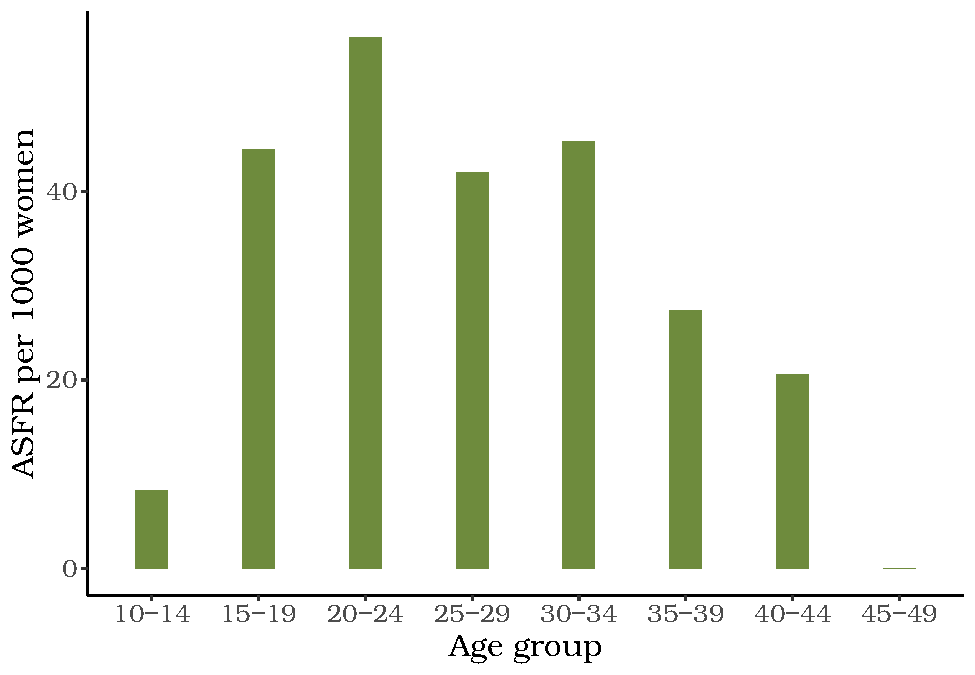
\includegraphics[width=0.8\linewidth]{mainfactsheet_files/figure-latex/unnamed-chunk-9-1}

We find the age specific fertility rate by looking at how many women in
a certain age group have had babies in a certain year. For example, we
can see that in 2019, for the women in the age group 15-19, 44 out of
every 1000 gave birth (if there had been over 1000 living in Agincourt.

\section{Deaths}

Below you can see the total number of deaths that occurred in the
Agincourt in 2019.

\begin{table}[ht]
\centering
\begin{tabularx}{\textwidth}{|l|C|}
  \rowcolor{igray} \hline
Category & Count \\ 
  \hline
Male Deaths &  16 \\ 
  Female Deaths &  21 \\ 
  Total Deaths &  37 \\ 
   \hline
\end{tabularx}
\end{table}

Below you can see the total number of death that occurred in the
Agincourt in 2019.

~\\
\begingroup \fontfamily{ppl}\fontsize{70}{70}\selectfont
\textbf{\textcolor{olive}{5}} \endgroup \begingroup
\fontsize{30}{30}\selectfont \textcolor{olive}{deaths} were

observed on average out

\textcolor{olive}{of every 1000 of the population}

in Agincourt in the year 2019 \endgroup

~\\
\hspace*{0.333em}

The crude death rate is obtained by comparing the number of deaths with
the total population. For every 1 000 people (all ages and both male and
female) living in Agincourt in the year of 2019, 5 deaths occured.

\section{Migration}
\subsection{Permanent migration patterns}

Below you can see how many people have moved into and out of Agincourt
permanently for the year of 2019.

\begin{table}[ht]
\centering
\begin{tabularx}{\textwidth}{|l|C|}
  \rowcolor{igray} \hline
Category & Count \\ 
  \hline
Male In-Migration &  21 \\ 
  Female In-Migration &  35 \\ 
   \hline
\end{tabularx}
\end{table}

\begin{table}[ht]
\centering
\begin{tabularx}{\textwidth}{|l|C|}
  \rowcolor{igray} \hline
Category & Count \\ 
  \hline
Male Out-Migration &  16 \\ 
  Female Out-Migration &  11 \\ 
   \hline
\end{tabularx}
\end{table}


\end{document}
